\section{Multiplicacion matrices}

Para este ejercicio se pedir diseñar un algoritmo de multiplicacion de matrices cuadradas y evaluar su eficiencia. El algoritmo diseñado es el siguiente:

El código de la función que implementa el algoritmo es el siguiente:

\begin{lstlisting}
  void multiplicar(int **a, int **b, int **result, int tam) {
    for(int i=0; i < tam; i++){ 
      for(int j=0; j < tam; j++){
        for(int k=0; k < tam; k++){
          result[i][j] += a[i][k]*b[k][j];
        }
      }
    }
  }
 \end{lstlisting}

\subsection{Analisis de eficiencia teoríco}

El analisis de eficiencia muestra que al ser tres bubles anidados el orden es $n^{3}$ y su desarrollo es el siguiente:
\begin{equation}
T(n)=\sum_{i=0}^{n}(\sum_{j=0}^{n}(\sum_{k=0}^{n}(1)))=n*\sum_{j=0}^{n}(\sum_{k=0}^{n}(1))=n^{2}*\sum_{k=0}^{n}(1)=n^{3}
\end{equation}



\subsection{Analisis empírico de eficiencie}

El analisis empírico en nuestra maquina arrojo los siguientes resultados, los cuales verifican el orden cúbico del algoritmo diseñado:

\begin{figure}[H]
  \centering
  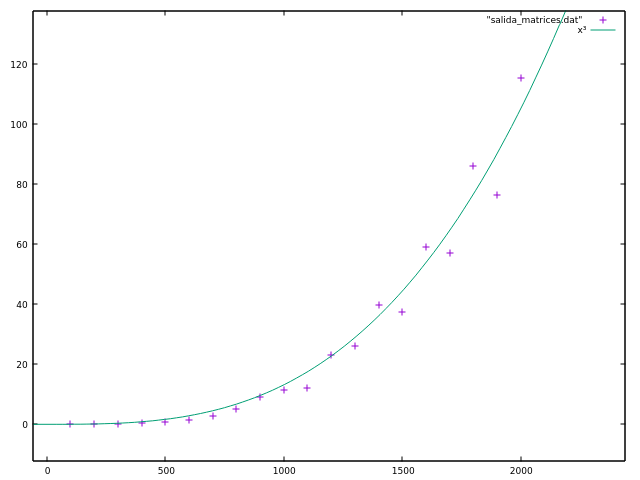
\includegraphics[width=0.5\textwidth]{./Imagenes/mult_matrices_ajustada.png}
  \caption{Grafica de las ejecuciones del algoritmo de multiplicación de matrices ajustada con la funcion $o(n^{3})$}
\end{figure}


Ademas se comprobo tambien como afecta la optimización a dicho algoritmo, lo cual se muestra en la siguiente gráfica.

\begin{figure}[H]
  \centering
  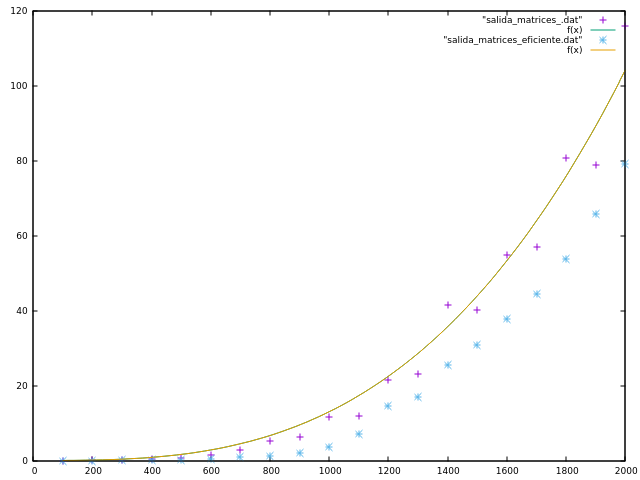
\includegraphics[width=0.5\textwidth]{./Imagenes/mult_matrices_optimizada_vs.png}
  \caption{Diferencia de tiempos para el algoritmo sin optimizar y el algoritmo optimizado}
\end{figure}

Donde se aprecia que para el tamaño de matriz máximo probado la diferencia es de 40 segundo, lo que en diversos casos puede representar un tiempo crítico, tambien es importante terner en cuanta que para mayores tamaños estas diferencias seguirian aumentando en funcion de $n^{3}$ por lo que seria conveniente diseñar algoritmos con un menor tiempo de ejecucion(se verá en el segundo cuatrimestre).
